\subsection{Topic Modeling} \label{sec:topciModeling}

Als Topic Modeling bezeichnet man Methoden, welche große Textdatenmengen in wenigen Dimensionen präsentieren \cite[3]{Kherwa2020}. Die wenigen Dimensionen sind wichtig, um die Topic Modeling-Methode visuell darstellen zu können. Im Grunde genommen suchen sich Topic Models Wörter, welche oft in einem \textbf{Korpus} miteinander zusammen verwendet werden, und fasst sie als Topics zusammen \cite{sense-topic-modelling-van-kessel}.

Es wird zwischen \textbf{probabilistischen} und \textbf{non-probabilistischen} bzw. \textbf{algebraischen Modellen} unterschieden \cite[3]{Kherwa2020}. Non-probabilistische Modelle oder algebraische Modelle basieren auf der \\\textbf{Matrix-Faktorisierung}. Probabilistische Modelle wurden später entwickelt, um algebraische Modelle zu verbessern, in dem man ihnen generative Modell-Herangehensweisen hinzugefügt hat.

Desweiteren unterscheidet man zwischen \textbf{supverised} und \textbf{unsupervised Learning}. Bei supervised Learning "füttert" man das Modell mit bereits bekannten \textbf{Trainingsdaten}, um es zu trainieren. \cite[186]{Plaue2021} Diese Trainingsdaten sind mit selbst vergebenen \textbf{Labels} versehen. Das Modell lernt somit, welche Eigenschaften von Daten mit welchen Labels zusammenhängen und kann (hoffentlich) nach dem Training selbst Daten korrekt labeln. Beim unsupervised Learning weiß man nicht im Vorhinein, was gesucht werden soll, dafür ist es schneller und billiger \cite{sense-topic-modelling-van-kessel}.

Die dritte Klassifizierung von Topic Modeling-Methoden ist die Tatsache, ob die Reihenfolge der Worte eine Rolle spielt oder nicht \cite[3]{Kherwa2020}. Bis zum Jahr 2006 wurden nur ein \textbf{\acrfull{ac:bow}} verwendet, in dem alle Wörter zusammengefasst werden. Die Reihenfolge spielt hierbei keine Rolle, nur die Anzahl der Vorkommnisse der Wörter ist relevant. Alternativen zum BOW sind Bigram- und N-gram-basierten Modelle, welche aber noch nicht so etabliert sind wie der BOW.

Folgende Grafik zeigt unterschiedliche Topic Modeling-Methoden auf \cite[3]{Kherwa2020}:

\begin{figure}
    \centering
    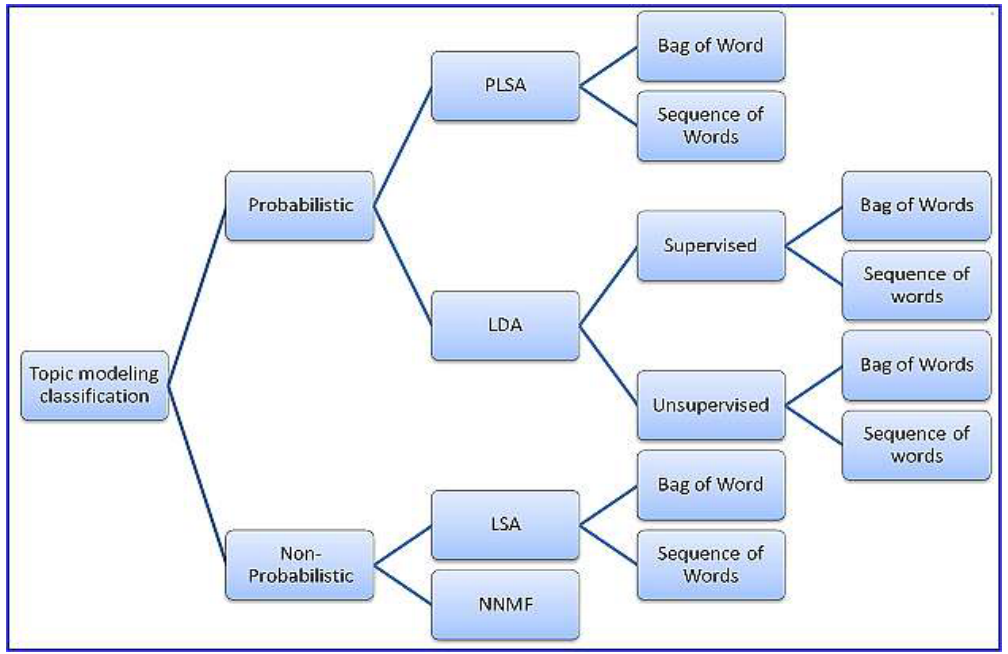
\includegraphics[scale=0.26]{images/dlengsteiner/topic-modeling-hierarchy.png}
    \caption{Hierarchische Klassifikation von Topic Modeling}
    \label{fig:topic-modeling-hierarchy}
\end{figure}

\newpage

So prakisch Topic Models sind, sie haben auch ihre Limitationen \cite{sense-topic-modelling-van-kessel}. Wie bereits erwähnt fassen Topic Models Wörter, welche häufig miteinander verwendet werden, als Topics zusammen.

Als Beispiel dient Abbildung \ref{fig:example-topic-modeling-1}. Im Topic 5 beispielsweise geht es darum, der Gemeinschaft uneigennützig etwas zurückzugeben. Das erkennt man an den Worten \textbf{giving}, \textbf{charitable}, \textbf{giving community} und \textbf{nonprofit}. Hier zeigt sich bereits die erste Limitation: Das Topic Model benennt das Topic nicht 'Giving back to society' oder dergleichen, sondern einfach nur Topic 5. Das Topic Model erkennt nämlich selbst nicht, was die Wörter bedeuten und in welchem Kontext sie miteinander zusammenhängen. Der Leser muss sich selbster Gedanken machen, worum es im Topic geht. Das ist für dieses Projekt etwas positives, da das engültige Produkt von Schülern und Lehrern verwendet wird, welche die Topics selbst im Unterricht interpretieren sollen.

\begin{figure}
    \centering
    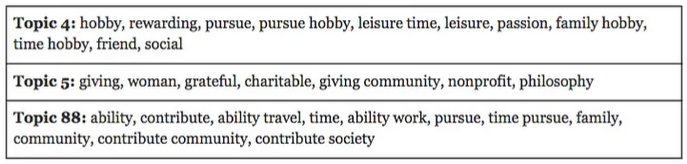
\includegraphics[scale=0.6]{images/dlengsteiner/example-topic-modeling-1}
    \caption{Beispiel eines Topic Models mit kontextuell unpassenden Wörtern}
    \label{fig:example-topic-modeling-1}
\end{figure}
Man betrachte wieder Abbildung \ref{fig:example-topic-modeling-1}. Die Wörter \textbf{woman} und \textbf{philosophy} aus Topic 5 passen nicht in das Schema von 'Giving back to society'. Daran erkennt man, dass Topic Models nicht garantieren können \cite{sense-topic-modelling-van-kessel}, dass die Wörter in einem Topic \textit{konzeptuell} miteinander verbunden sind. Diese Wörter erscheinen vielleicht harmlos, können aber ein Problem darstellen, wenn es darum geht, zu sagen, wie oft das Topic im Korpus vorkommt. Nimmt man die obigen unpassenden Wörter aus dem Topic heraus, bleibt vielleicht nur noch einen Bruchteil der Vorkommnisse des Topics im Korpus übrig.

Eine Weitere Limitation ist die Tatsache, dass die Anzahl der Topics vorgegeben werden muss und nicht vom Topic model erkannt wird \cite{sense-topic-modelling-van-kessel}. Daher kann es oft passieren, dass, egal wie viele Topics man ausgewählt hat, Topics bekommt, welche zu genau oder ungenau sind.

\begin{figure}
    \centering
    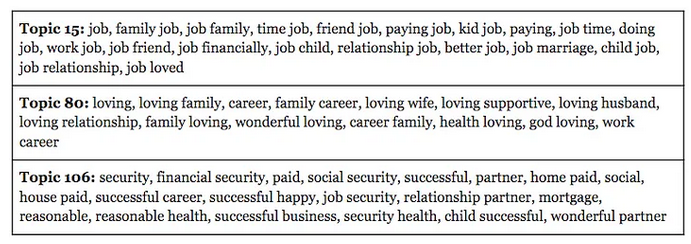
\includegraphics[scale=0.6]{images/dlengsteiner/example-topic-modeling-2}
    \caption{Beispiel eines Topic Models mit zu (un)genauen Topics}
    \label{fig:example-topic-modeling-2}
\end{figure}
Wie in Abbildung \ref{fig:example-topic-modeling-2} zu sehen, fasst das Topic 106 mehrere konzeptuelle Themen in ein Topic zusammen. Diese Topics könnten sein: security, finance, health, relationships, success. Solche Topics nennt man \textbf{undercooked Topics} \cite{sense-topic-modelling-van-kessel}, also Topics, welche nicht fokussiert genug sind.

Im selben Topic Model gibt es aber auch das Topic 15, welches \textit{zu genau} ist, also \textbf{overcooked}. Jedes Topic erwähnt das Wort \textbf{job}. Wörter, die dazu passen, wie \textbf{career} oder \textbf{work}, sind nicht im Topic 15 vorhanden. Diese Wörter kommen jedoch im Topic 108 vor. Um diese 'falsch gekochten' Topics zu reparieren, muss man die Anzahl der Topics verändern. Das könnte jedoch zu weiteren Problemen führen.

Um manche dieser Limitationen zu überwinden \cite{sense-topic-modelling-van-kessel}, müsste man den durch das Finden der Traingsdaten zeitaufwändigen und teuren Prozess des supervised Learnings gehen. Der andere Weg wäre, KIs anzuwenden. Mit letzterer Thematik beschäftigt sich das Kapitel \nameref{sec:ai-recognition}).

\subsubsection{\acrfull{ac:lsa}}

LSA ist eine algebraische Topic Modeling-Methode und basiert auf der \textbf{Single Value Decomposition (SVD)} \cite[4]{Kherwa2020}. Das theoretische Fundament für LSA besagt, dass Wörter, welche eine ähnliche Bedeutung haben, nahe aneinander liegen, was ihre Verwendung betrifft. Um diese Ähnlichkeiten zu finden, verwendet man eine Vektor-Repräsentation des Textes.

LSA verwendet SVD, um die Daten umzuorganisieren \cite[174]{topicmodelsurvey_padmaja}. SVD verwendet eine Matrix, um die Dimensionen im Vektorraum zu re-konfigurieren und neu zu berechnen. Diese Dimensionen werden nach Wichtigkeit geordnet.

Man geht folgendermaßen mit LSA vor:
\begin{enumerate}
    \item Man erstellt eine \textbf{Term Frequency Matrix}, welche die Vorkommnisse jedes Begriffs enthält\cite[174]{topicmodelsurvey_padmaja}\cite[4]{Kherwa2020}. Diese wird als $A$ bezeichnet.
    \item Jedes Wort bekommt durch eine Gewichtungs-Funktion eine Wichtigkeit für das Dokument und den gesamten Korpus \cite[4]{Kherwa2020}. Wörter, welche häufig und in vielen Dokumenten des Korpus vorkommen, bekommen ein niedrige Wichtigkeit. Wörtern, welche in nur wenigen Dokumenten vorkommen, wird eine höere Wichtigkeit zugeschrieben.
    \item Danach wendet man SVD an \cite[4]{Kherwa2020}. Die Matrix $A$ wird folgendermaßen dekomposiert:
    \[
    A=U\Sigma V^T
    \]
    Hierbei gilt: $U$ und $V$ sind orthogonale Matrizen, und $\Sigma$ ist eine diagonale Matrix.
    
    Orthogonale Matrizen sind Matrizen, wessen Produkt mit ihrer transponierten Matrix die Einheitsmatrix $I$ ergibt, also:
    \[
    U\cdot U^T = I = \begin{pmatrix}
        1 & 0 \\ 0 & 1
    \end{pmatrix}
    \]
    Die Diagonale Matrix $\Sigma$ hat nur Werte auf der Hauptdiagonalen \cite[4]{Kherwa2020}:
    \[
    \Sigma=\begin{pmatrix}
        \sigma_1 & 0 & \cdots\\
        \cdots & \sigma_2 & \cdots\\
        \cdots & 0 & \sigma_k
    \end{pmatrix}
    \]
    \item Danach stutzt man die Matrix $A$ als Matrix $A_k$ \cite[4]{Kherwa2020}. 
\end{enumerate}

\subsubsection{\acrfull{ac:nnmf}}

Negative Zahlen in Datensätzen stellen ein Problem für Topic Models dar \cite[4]{Kherwa2020}, da negative Zahlen oft nicht realitätskonform sind. \acrshort{ac:nnmf} adressiert dieses Problem, indem es nichtnegative Beschränkungen auf das Datenmodell platziert.

Die Grundlegende Idee von \acrshort{ac:nnmf} ist es, eine nichtnegative Matrix $B$ in die nichtnegativen Faktoren $V$ und $H$ zu zerlegen \cite[4]{Kherwa2020}:
\[
B=VH+C\quad\quad V\geq 0,\quad H\geq 0
\]
Die Zahl $C$ stellt hierbei ein unvermeidbares Rauschen dar.

NNMF hat einige Anwendungsbereiche \cite[4]{Kherwa2020}, unter anderem Dimensionsreduktion, Mustererkennung, Bildverarbeitung und das für dieses Projekt am relevantesten, Sprachmodellierung.

\subsubsection{\acrfull{ac:plsa}}

PLSA ist der probabilistische Nachgfolger von LSA, was bedeutet, dass man den Vorgänger mittels einem probabilitsichen Ansatzes durch die Verwendung eines generativen Modells verbessern möchte \cite[148]{Alghamdi2015}.

Das Hauptobjektiv von PLSA ist die Erkennung und Differenzierung von Kontexts einer Wortverwendung ohne einen Rückgriff auf ein Wörterbuch oder Wörtersammlung \cite[148]{Alghamdi2015}. Das erlaubt es PLSA, verschiedene Bedeutungen des selben Wortes zu erkennen. Desweiteren kann es Wörter gruppieren, welche in einem gemeinsamen Kontext verwendet wurden.

\subsubsection{\acrfull{ac:lda}}

LDA ist eine Topic Modeling-Methode des unsupervised Learnings \cite[149]{Alghamdi2015}. Es baut auf statistischen (Bayesian) Topic Models auf und findet sehr weit verbreitet Anwendung, sei es von automatisierten Bewertungen bis als Maßnahme gegen Phishing-Mails \cite[150]{Alghamdi2015}.

LDA teilt ein Dokument in Topics auf, wobei jedes Topic eine diskrete Wahrscheinlichkeitsverteilung ist, welche definiert, wie wahrscheinlich es ist, das ein Wort in diesem Topic vorkommt \cite[149]{Alghamdi2015}. Für LDA ist das Dokument nur ein Bag of Words (siehe \ref{sec:topciModeling}

Der Vorteil von LDA im Vergleich zu LSA und PLSA besteht in der Dimensionsreduktion \cite[175]{topicmodelsurvey_padmaja}, welche es LDA erlaubt, in komplizierteren Methoden verwendet zu werden. Wenn man jedoch viele Dokumente, lange Dokumente oder sehr viele Topics mit LDA bearbeiten möchte, stößt dieses Modell auf seine Grenzen. Außerdem ist LDA nicht in der Lage, Korrelationen zwischen Topics zu erkennen.

\subsubsection{\acrfull{ac:ctm}}

Aus diesem Grund wurde CTM entwickelt, eine Variante von LDA \cite[175]{topicmodelsurvey_padmaja}, welche als Antwort auf die Inabilität von LDA, Korrelationen zwischen Topics zu sehen, entwickelt wurde.

Dokumente teilen sich gemischte Modelle \cite[175]{topicmodelsurvey_padmaja}, wessen Proportionen als zufällige Variablen gehandhabt werden, welche spezifisch für jedes Dokument sind. Jedes Dokument wird als Kombination von Topics mit unterschiedlichen Proportionen gesehen.

CTM verwendet die logistische Normalverteilung \cite[175]{topicmodelsurvey_padmaja}, um die versteckte Kompositionen von Topics und deren Proportionen zu modellieren. Das führt jedoch dazu, dass CTM ungeeignet für kompliziertere Methoden ist.

\subsubsection{\acrfull{ac:dtm}}

DTM ist eine Erweiterung von LDA \cite[175]{topicmodelsurvey_padmaja}. LDA sieht nämlich alle Dokumente als BOWs an (siehe \ref{sec:topciModeling}), wodurch LDA annimmt, dass diese Dokumente von den selben Topics gezogen wurden.

DTM hingegen erlaubt es, dass die Verteilung der Topics auf unterschiedliche Dokumente \cite[175]{topicmodelsurvey_padmaja} sowie die Verteilung der Wörter in den Topics unterschiedlich analysiert werden kann.

Mittels der Verwendung von Metadaten der Dokumente ist DTM in der Lage, Topics über einen Zeitraum zu erkennen \cite[175]{topicmodelsurvey_padmaja}. Darin liegt der Vorteil gegenüber anderen probabilistischen Topic Modeling-Methoden. DTM hat aber auch Limitationen. Einerseits erlaubt es nur eine fixierte Anzahl von Topics. Andererseits ist es nicht sinnvoll, die Genauigkeit der Zeit signifikant zu erhöhen, da sonst die Komplexität der Variationen und deren Schlussfolgerungen so hoch wird, dass die Rechenleistung nicht mitkommt.

\subsubsection{\acrfull{ac:hlda}}

LDA stellt Topics als einfache Struktur dar \cite[175]{topicmodelsurvey_padmaja} und ist somit nicht in der Lage, Beziehungen zwischen Topics zu finden. HLDA löst dies, indem die Topics in einer hierarchischen Baumstruktur dargestellt werden. Je absktrakter ein Topic, desto näher befindet es sich bei der Wurzel des Baumes.

HLDA verwendet einen \textbf{Nested Chinese Restaurant Process (nested CRP)} \cite[175]{topicmodelsurvey_padmaja}, um eine gemischte Verteilung der Topics zu kreieren. Diesen nested CRP verwendet man danach wieder, um die Topics zu einer Hierarchie zusammenzuführen. Um Wörter für die Topics zu finden, sucht HLDA sich zuerst ein Topic nach dessen Verteilung aus und generiert dann Wörter nach der Wortverteilung des Topics.